\documentclass[11pt, a4paper]{article}\usepackage[]{graphicx}\usepackage[]{xcolor}
% maxwidth is the original width if it is less than linewidth
% otherwise use linewidth (to make sure the graphics do not exceed the margin)
\makeatletter
\def\maxwidth{ %
  \ifdim\Gin@nat@width>\linewidth
    \linewidth
  \else
    \Gin@nat@width
  \fi
}
\makeatother

\definecolor{fgcolor}{rgb}{0.345, 0.345, 0.345}
\newcommand{\hlnum}[1]{\textcolor[rgb]{0.686,0.059,0.569}{#1}}%
\newcommand{\hlstr}[1]{\textcolor[rgb]{0.192,0.494,0.8}{#1}}%
\newcommand{\hlcom}[1]{\textcolor[rgb]{0.678,0.584,0.686}{\textit{#1}}}%
\newcommand{\hlopt}[1]{\textcolor[rgb]{0,0,0}{#1}}%
\newcommand{\hlstd}[1]{\textcolor[rgb]{0.345,0.345,0.345}{#1}}%
\newcommand{\hlkwa}[1]{\textcolor[rgb]{0.161,0.373,0.58}{\textbf{#1}}}%
\newcommand{\hlkwb}[1]{\textcolor[rgb]{0.69,0.353,0.396}{#1}}%
\newcommand{\hlkwc}[1]{\textcolor[rgb]{0.333,0.667,0.333}{#1}}%
\newcommand{\hlkwd}[1]{\textcolor[rgb]{0.737,0.353,0.396}{\textbf{#1}}}%
\let\hlipl\hlkwb

\usepackage{framed}
\makeatletter
\newenvironment{kframe}{%
 \def\at@end@of@kframe{}%
 \ifinner\ifhmode%
  \def\at@end@of@kframe{\end{minipage}}%
  \begin{minipage}{\columnwidth}%
 \fi\fi%
 \def\FrameCommand##1{\hskip\@totalleftmargin \hskip-\fboxsep
 \colorbox{shadecolor}{##1}\hskip-\fboxsep
     % There is no \\@totalrightmargin, so:
     \hskip-\linewidth \hskip-\@totalleftmargin \hskip\columnwidth}%
 \MakeFramed {\advance\hsize-\width
   \@totalleftmargin\z@ \linewidth\hsize
   \@setminipage}}%
 {\par\unskip\endMakeFramed%
 \at@end@of@kframe}
\makeatother

\definecolor{shadecolor}{rgb}{.97, .97, .97}
\definecolor{messagecolor}{rgb}{0, 0, 0}
\definecolor{warningcolor}{rgb}{1, 0, 1}
\definecolor{errorcolor}{rgb}{1, 0, 0}
\newenvironment{knitrout}{}{} % an empty environment to be redefined in TeX

\usepackage{alltt}

\usepackage[top=1 in, bottom = 1 in, left = 1 in, right = 1 in ]{geometry}

\usepackage{amsmath, amssymb, amsfonts}
\usepackage{enumerate}
\usepackage{utfsym}

\title{Linear Models with R - Julian J. Faraway}
\author{Ananda Biswas}
\date{}
\IfFileExists{upquote.sty}{\usepackage{upquote}}{}
\begin{document}

\maketitle

\begin{center}
  \section*{Chapter 1 - Exercise 1}
\end{center}



$\bullet$ loading the library
\begin{knitrout}
\definecolor{shadecolor}{rgb}{0.969, 0.969, 0.969}\color{fgcolor}\begin{kframe}
\begin{alltt}
\hlkwd{library}\hlstd{(faraway)}
\end{alltt}


{\ttfamily\noindent\color{warningcolor}{\#\# Warning: package 'faraway' was built under R version 4.2.3}}\end{kframe}
\end{knitrout}

$\bullet$ loading the data set
\begin{knitrout}
\definecolor{shadecolor}{rgb}{0.969, 0.969, 0.969}\color{fgcolor}\begin{kframe}
\begin{alltt}
\hlkwd{data}\hlstd{(}\hlstr{"teengamb"}\hlstd{)}

\hlstd{my_data} \hlkwb{<-} \hlstd{teengamb}
\end{alltt}
\end{kframe}
\end{knitrout}

$\bullet$ description of the data
\begin{knitrout}
\definecolor{shadecolor}{rgb}{0.969, 0.969, 0.969}\color{fgcolor}\begin{kframe}
\begin{alltt}
\hlkwd{`?`}\hlstd{(teengamb)}
\end{alltt}


{\ttfamily\noindent\itshape\color{messagecolor}{\#\# starting httpd help server ... done}}\end{kframe}
\end{knitrout}

$\bullet$ doing sanity checks
\begin{knitrout}
\definecolor{shadecolor}{rgb}{0.969, 0.969, 0.969}\color{fgcolor}\begin{kframe}
\begin{alltt}
\hlkwd{dim}\hlstd{(my_data)}
\end{alltt}
\begin{verbatim}
## [1] 47  5
\end{verbatim}
\end{kframe}
\end{knitrout}

\begin{knitrout}
\definecolor{shadecolor}{rgb}{0.969, 0.969, 0.969}\color{fgcolor}\begin{kframe}
\begin{alltt}
\hlkwd{names}\hlstd{(my_data)}
\end{alltt}
\begin{verbatim}
## [1] "sex"    "status" "income" "verbal" "gamble"
\end{verbatim}
\end{kframe}
\end{knitrout}

\begin{knitrout}
\definecolor{shadecolor}{rgb}{0.969, 0.969, 0.969}\color{fgcolor}\begin{kframe}
\begin{alltt}
\hlkwd{head}\hlstd{(my_data)}
\end{alltt}
\begin{verbatim}
##   sex status income verbal gamble
## 1   1     51   2.00      8    0.0
## 2   1     28   2.50      8    0.0
## 3   1     37   2.00      6    0.0
## 4   1     28   7.00      4    7.3
## 5   1     65   2.00      8   19.6
## 6   1     61   3.47      6    0.1
\end{verbatim}
\end{kframe}
\end{knitrout}

\begin{knitrout}
\definecolor{shadecolor}{rgb}{0.969, 0.969, 0.969}\color{fgcolor}\begin{kframe}
\begin{alltt}
\hlkwd{tail}\hlstd{(my_data)}
\end{alltt}
\begin{verbatim}
##    sex status income verbal gamble
## 42   0     61  15.00      9   69.7
## 43   0     75   3.00      8   13.3
## 44   0     66   3.25      9    0.6
## 45   0     62   4.94      6   38.0
## 46   0     71   1.50      7   14.4
## 47   0     71   2.50      9   19.2
\end{verbatim}
\end{kframe}
\end{knitrout}

$\bullet$ From the description we see that, sex is a categorical variable.
\begin{knitrout}
\definecolor{shadecolor}{rgb}{0.969, 0.969, 0.969}\color{fgcolor}\begin{kframe}
\begin{alltt}
\hlstd{my_data}\hlopt{$}\hlstd{sex} \hlkwb{<-} \hlkwd{factor}\hlstd{(my_data}\hlopt{$}\hlstd{sex)}

\hlkwd{levels}\hlstd{(my_data}\hlopt{$}\hlstd{sex)} \hlkwb{<-} \hlkwd{c}\hlstd{(}\hlstr{"male"}\hlstd{,} \hlstr{"female"}\hlstd{)}
\end{alltt}
\end{kframe}
\end{knitrout}


\begin{knitrout}
\definecolor{shadecolor}{rgb}{0.969, 0.969, 0.969}\color{fgcolor}\begin{kframe}
\begin{alltt}
\hlkwd{class}\hlstd{(my_data}\hlopt{$}\hlstd{sex)}
\end{alltt}
\begin{verbatim}
## [1] "factor"
\end{verbatim}
\begin{alltt}
\hlkwd{class}\hlstd{(my_data}\hlopt{$}\hlstd{status)}
\end{alltt}
\begin{verbatim}
## [1] "integer"
\end{verbatim}
\begin{alltt}
\hlkwd{class}\hlstd{(my_data}\hlopt{$}\hlstd{income)}
\end{alltt}
\begin{verbatim}
## [1] "numeric"
\end{verbatim}
\begin{alltt}
\hlkwd{class}\hlstd{(my_data}\hlopt{$}\hlstd{verbal)}
\end{alltt}
\begin{verbatim}
## [1] "integer"
\end{verbatim}
\begin{alltt}
\hlkwd{class}\hlstd{(my_data}\hlopt{$}\hlstd{gamble)}
\end{alltt}
\begin{verbatim}
## [1] "numeric"
\end{verbatim}
\end{kframe}
\end{knitrout}


\begin{knitrout}
\definecolor{shadecolor}{rgb}{0.969, 0.969, 0.969}\color{fgcolor}\begin{kframe}
\begin{alltt}
\hlkwd{summary}\hlstd{(my_data)}
\end{alltt}
\begin{verbatim}
##      sex         status          income           verbal          gamble     
##  male  :28   Min.   :18.00   Min.   : 0.600   Min.   : 1.00   Min.   :  0.0  
##  female:19   1st Qu.:28.00   1st Qu.: 2.000   1st Qu.: 6.00   1st Qu.:  1.1  
##              Median :43.00   Median : 3.250   Median : 7.00   Median :  6.0  
##              Mean   :45.23   Mean   : 4.642   Mean   : 6.66   Mean   : 19.3  
##              3rd Qu.:61.50   3rd Qu.: 6.210   3rd Qu.: 8.00   3rd Qu.: 19.4  
##              Max.   :75.00   Max.   :15.000   Max.   :10.00   Max.   :156.0
\end{verbatim}
\end{kframe}
\end{knitrout}

\newpage

$\bullet$ Now we shall do a box-plot for gambling expenditure and sex.
\begin{knitrout}
\definecolor{shadecolor}{rgb}{0.969, 0.969, 0.969}\color{fgcolor}\begin{kframe}
\begin{alltt}
\hlkwd{boxplot}\hlstd{(gamble} \hlopt{~} \hlstd{sex, my_data,} \hlkwc{main} \hlstd{=} \hlstr{"Expenditure on gambling in Pounds per year"}\hlstd{)}
\end{alltt}
\end{kframe}
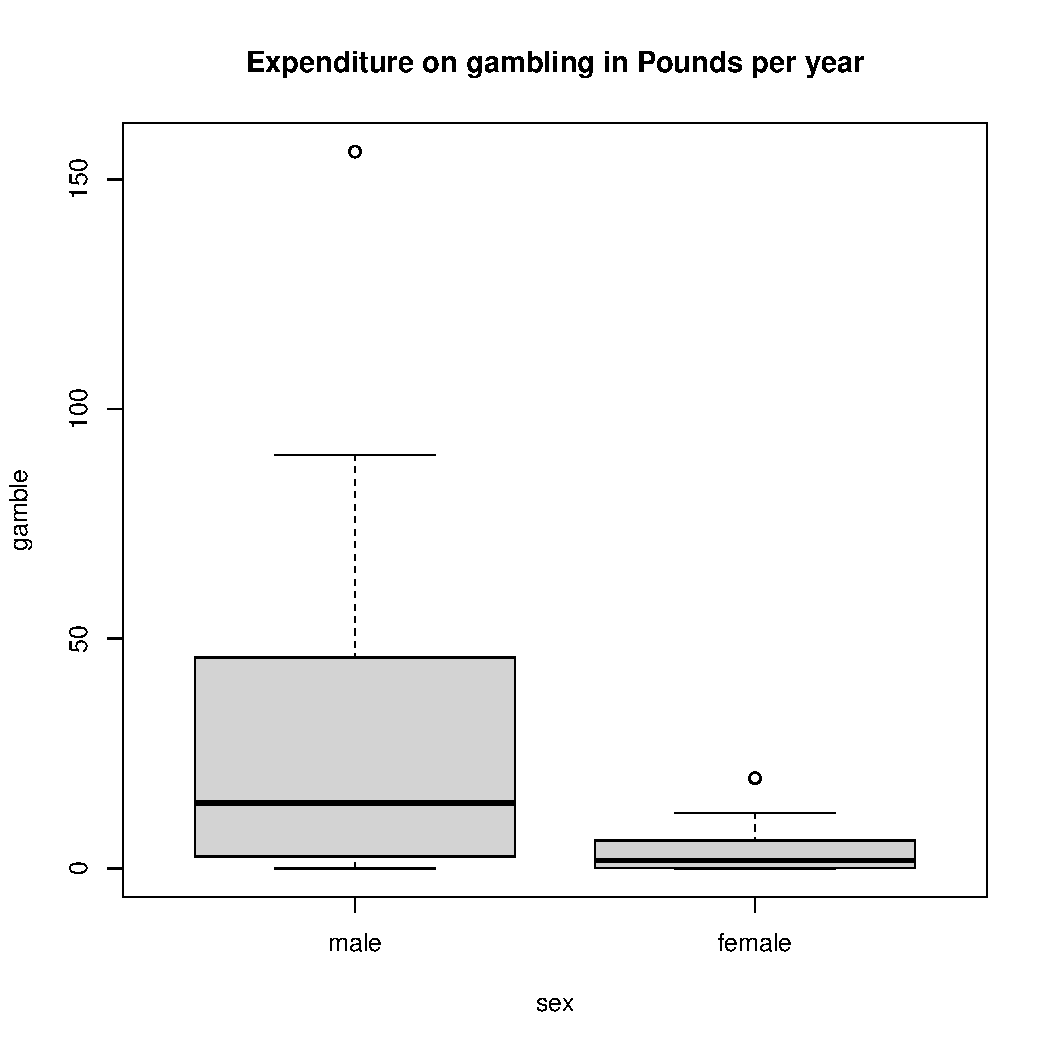
\includegraphics[width=\maxwidth]{figure/unnamed-chunk-11-1} 
\end{knitrout}

$\usym{261E}$ \textcolor{blue}{We see that expenditure on gambling by men is much higher than that by women.} \\

\newpage

$\bullet$ Now we shall see the correlation matrix.
\begin{knitrout}
\definecolor{shadecolor}{rgb}{0.969, 0.969, 0.969}\color{fgcolor}\begin{kframe}
\begin{alltt}
\hlkwd{cor}\hlstd{(my_data[}\hlopt{-}\hlnum{1}\hlstd{])}
\end{alltt}
\begin{verbatim}
##             status     income     verbal      gamble
## status  1.00000000 -0.2750340  0.5316102 -0.05042081
## income -0.27503402  1.0000000 -0.1755707  0.62207690
## verbal  0.53161022 -0.1755707  1.0000000 -0.22005619
## gamble -0.05042081  0.6220769 -0.2200562  1.00000000
\end{verbatim}
\end{kframe}
\end{knitrout}

A helpful visualization of the correlation matrix is as follows :
\begin{knitrout}
\definecolor{shadecolor}{rgb}{0.969, 0.969, 0.969}\color{fgcolor}\begin{kframe}
\begin{alltt}
\hlkwd{library}\hlstd{(corrplot)}
\end{alltt}


{\ttfamily\noindent\color{warningcolor}{\#\# Warning: package 'corrplot' was built under R version 4.2.3}}

{\ttfamily\noindent\itshape\color{messagecolor}{\#\# corrplot 0.92 loaded}}\end{kframe}
\end{knitrout}

\begin{knitrout}
\definecolor{shadecolor}{rgb}{0.969, 0.969, 0.969}\color{fgcolor}\begin{kframe}
\begin{alltt}
\hlkwd{corrplot}\hlstd{(}\hlkwd{cor}\hlstd{(my_data[}\hlopt{-}\hlnum{1}\hlstd{]),} \hlkwc{method} \hlstd{=} \hlstr{"number"}\hlstd{,}
    \hlkwc{type} \hlstd{=} \hlstr{"upper"}\hlstd{,} \hlkwc{tl.srt} \hlstd{=} \hlnum{45}\hlstd{,} \hlkwc{bg} \hlstd{=} \hlstr{"red"}\hlstd{,}
    \hlkwc{outline} \hlstd{=} \hlnum{TRUE}\hlstd{,} \hlkwc{tl.col} \hlstd{=} \hlstr{"blue"}\hlstd{)}
\end{alltt}
\end{kframe}
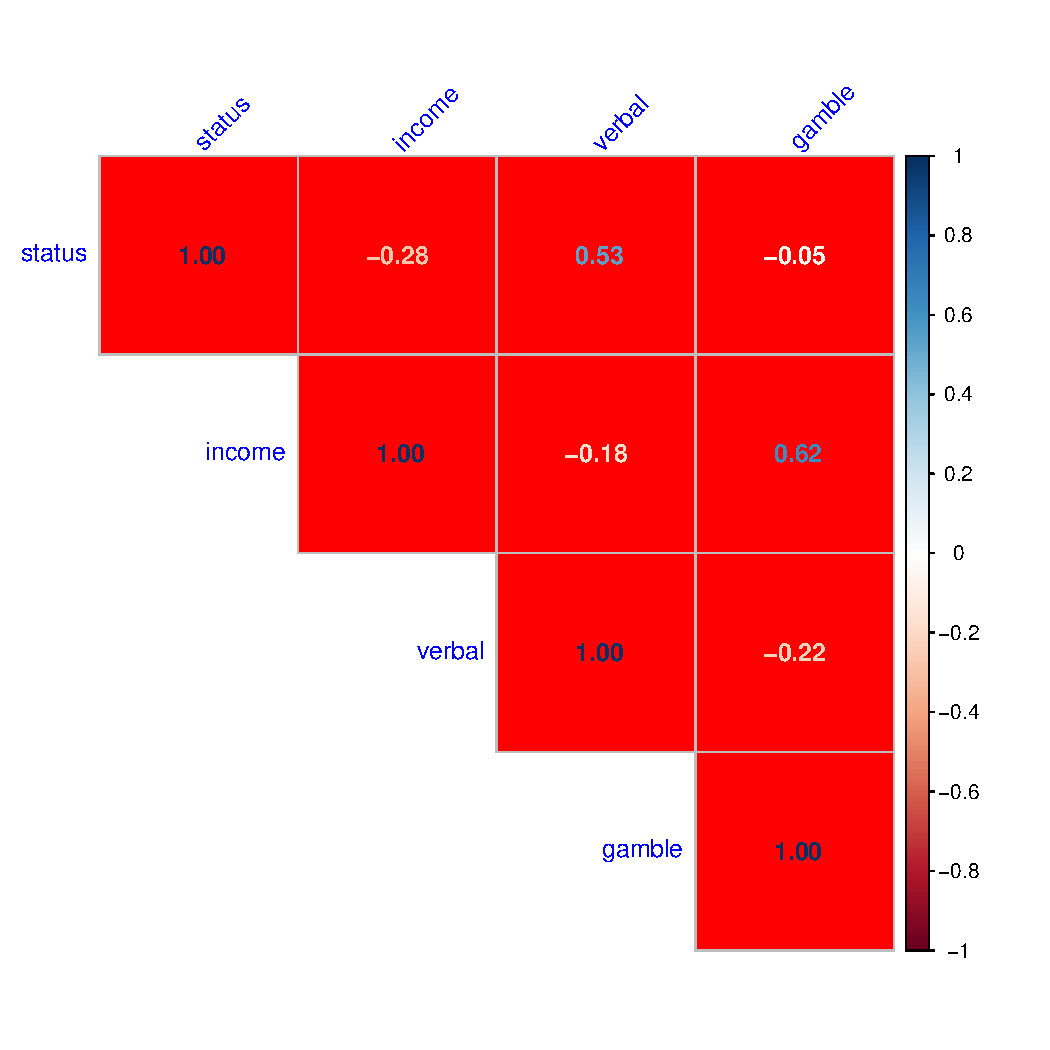
\includegraphics[width=\maxwidth]{figure/unnamed-chunk-14-1} 
\end{knitrout}

\newpage

We see that \textbf{status} and \textbf{gamble} have a slightly negative correlation. Let's see their scatterplot.
\begin{knitrout}
\definecolor{shadecolor}{rgb}{0.969, 0.969, 0.969}\color{fgcolor}\begin{kframe}
\begin{alltt}
\hlkwd{plot}\hlstd{(gamble} \hlopt{~} \hlstd{status,} \hlkwc{data} \hlstd{= my_data)}
\end{alltt}
\end{kframe}
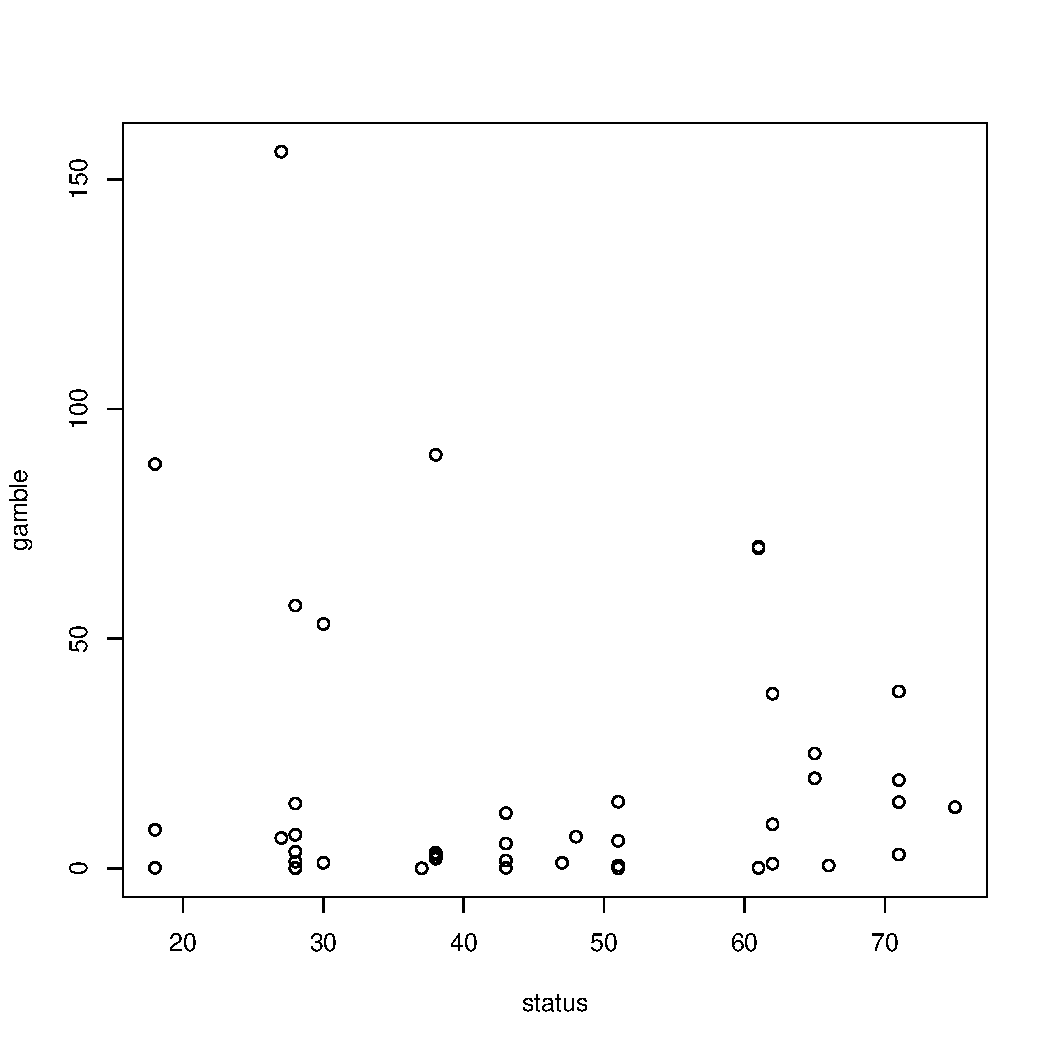
\includegraphics[width=\maxwidth]{figure/unnamed-chunk-15-1} 
\end{knitrout}

\newpage

$\usym{261E}$ \textcolor{blue}{We see that \textbf{income} and \textbf{gamble} have a correlation of $0.62$, a pretty decent correlation, implying that, people with higher income spend more on gambling. Let's see their scatterplot.}
\begin{knitrout}
\definecolor{shadecolor}{rgb}{0.969, 0.969, 0.969}\color{fgcolor}\begin{kframe}
\begin{alltt}
\hlkwd{plot}\hlstd{(gamble} \hlopt{~} \hlstd{income,} \hlkwc{data} \hlstd{= my_data)}
\end{alltt}
\end{kframe}
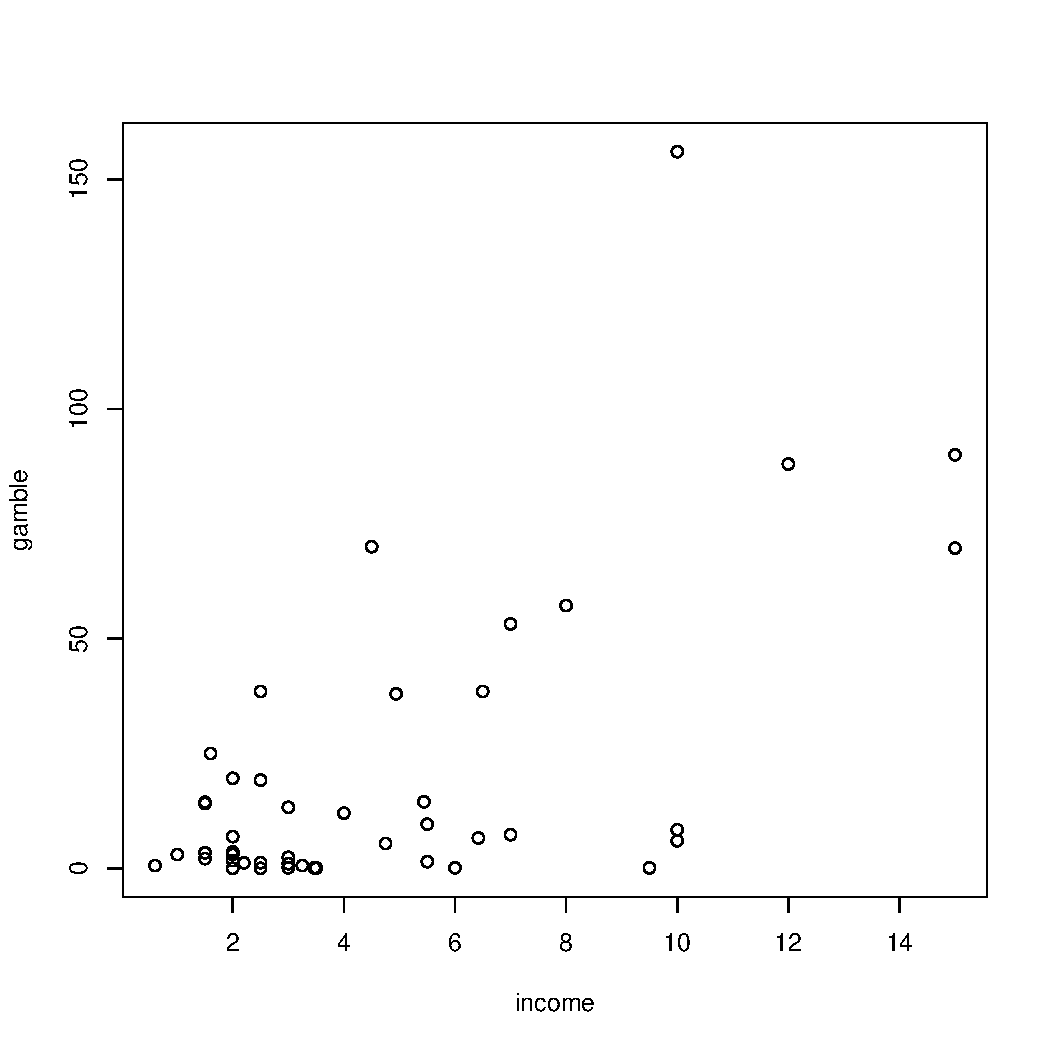
\includegraphics[width=\maxwidth]{figure/unnamed-chunk-16-1} 
\end{knitrout}

\newpage

$\usym{261E}$ \textcolor{blue}{\textbf{verbal} and \textbf{gamble} have a negative correlation. The variable \textit{verbal} is the score in words out of 12 correctly defined. This may be interpreted as a measure of literacy. That means literacy and expenditure in gambling are negatively correlated. Literate people tend to spend less on gambling, while less literate people end up spending more on gambling. Let's see their scatterplot.}
\begin{knitrout}
\definecolor{shadecolor}{rgb}{0.969, 0.969, 0.969}\color{fgcolor}\begin{kframe}
\begin{alltt}
\hlkwd{plot}\hlstd{(gamble} \hlopt{~} \hlstd{verbal,} \hlkwc{data} \hlstd{= my_data)}
\end{alltt}
\end{kframe}
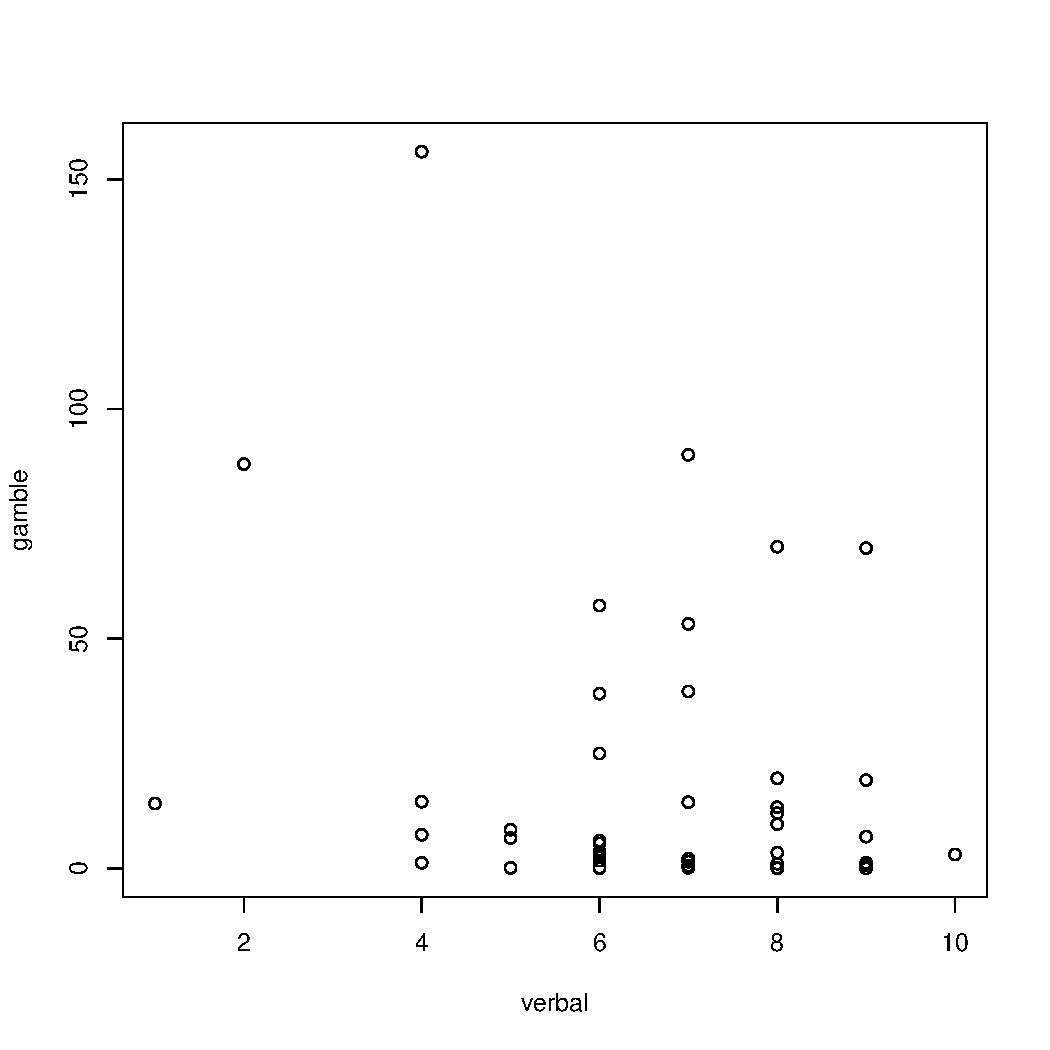
\includegraphics[width=\maxwidth]{figure/unnamed-chunk-17-1} 
\end{knitrout}

\newpage

The variable \textit{verbal} is a discrete valued variable. A box-plot may be helpful to see the relation between \textit{verbal} and \textit{gamble}.
\begin{knitrout}
\definecolor{shadecolor}{rgb}{0.969, 0.969, 0.969}\color{fgcolor}\begin{kframe}
\begin{alltt}
\hlkwd{boxplot}\hlstd{(gamble} \hlopt{~} \hlkwd{factor}\hlstd{(verbal),} \hlkwc{data} \hlstd{= my_data,}
    \hlkwc{xlab} \hlstd{=} \hlstr{"Number of words correctly defined"}\hlstd{,}
    \hlkwc{ylab} \hlstd{=} \hlstr{"Expenditure on Gamble"}\hlstd{)}
\end{alltt}
\end{kframe}
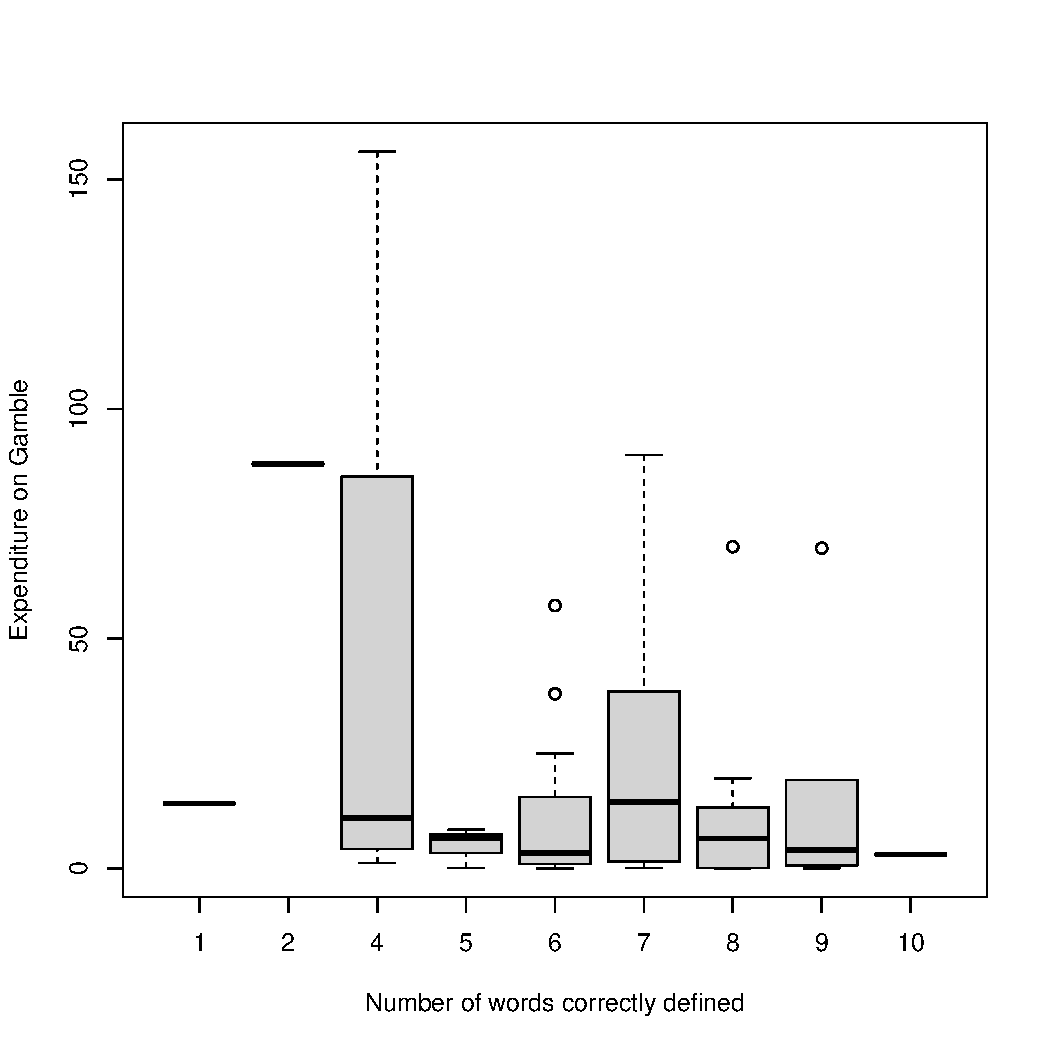
\includegraphics[width=\maxwidth]{figure/unnamed-chunk-18-1} 
\end{knitrout}

\newpage

We also see a positive correlation between \textit{status} and \textit{verbal}.
\begin{knitrout}
\definecolor{shadecolor}{rgb}{0.969, 0.969, 0.969}\color{fgcolor}\begin{kframe}
\begin{alltt}
\hlkwd{boxplot}\hlstd{(status} \hlopt{~} \hlkwd{factor}\hlstd{(verbal),} \hlkwc{data} \hlstd{= my_data,}
    \hlkwc{xlab} \hlstd{=} \hlstr{"Number of words correctly defined"}\hlstd{,}
    \hlkwc{ylab} \hlstd{=} \hlstr{"Expenditure on Gamble"}\hlstd{)}
\end{alltt}
\end{kframe}
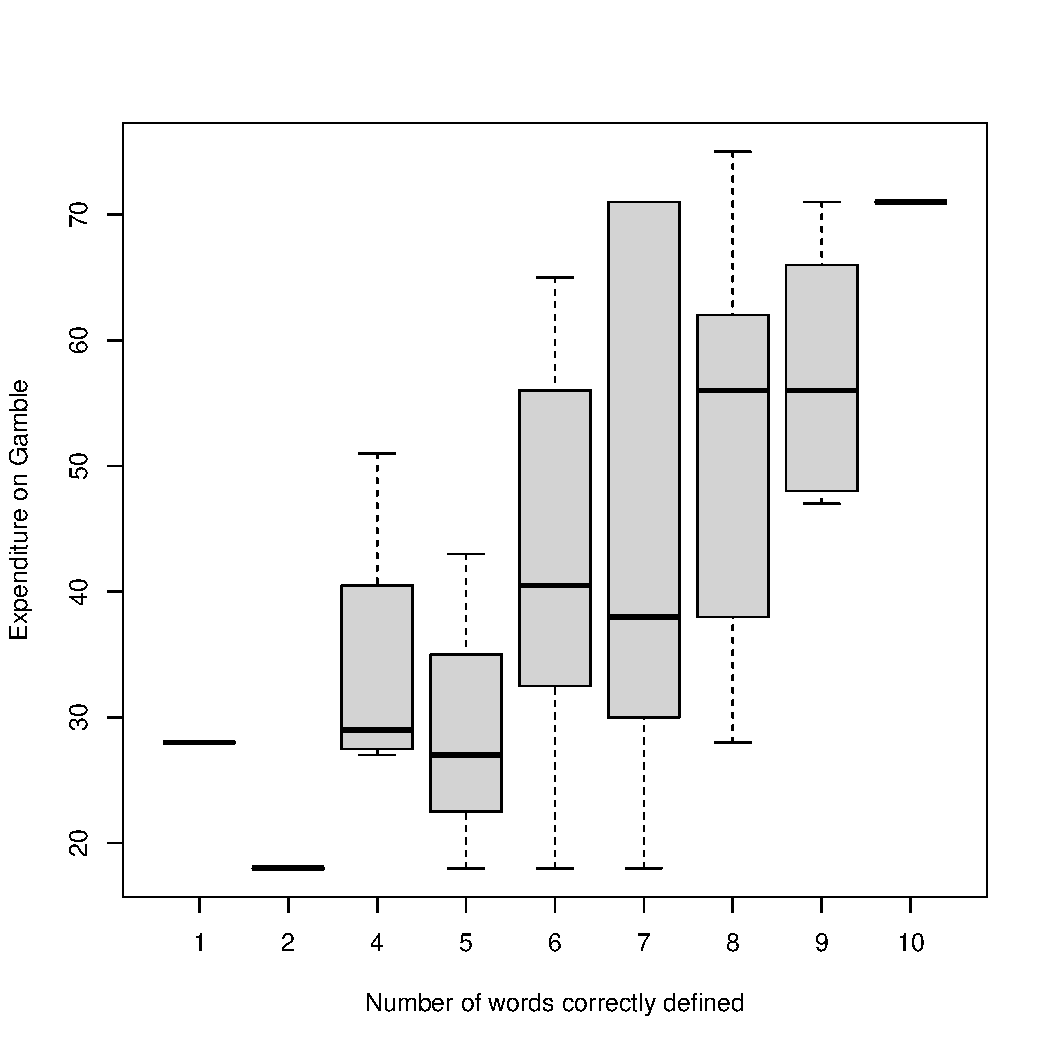
\includegraphics[width=\maxwidth]{figure/unnamed-chunk-19-1} 
\end{knitrout}

$\bullet$ Average spending on gambling by men is :
\begin{knitrout}
\definecolor{shadecolor}{rgb}{0.969, 0.969, 0.969}\color{fgcolor}\begin{kframe}
\begin{alltt}
\hlkwd{mean}\hlstd{(my_data}\hlopt{$}\hlstd{gamble[}\hlkwd{which}\hlstd{(my_data}\hlopt{$}\hlstd{sex} \hlopt{==}
    \hlstr{"male"}\hlstd{)])}
\end{alltt}
\begin{verbatim}
## [1] 29.775
\end{verbatim}
\end{kframe}
\end{knitrout}

$\bullet$ Average spending on gambling by women is :
\begin{knitrout}
\definecolor{shadecolor}{rgb}{0.969, 0.969, 0.969}\color{fgcolor}\begin{kframe}
\begin{alltt}
\hlkwd{mean}\hlstd{(my_data}\hlopt{$}\hlstd{gamble[}\hlkwd{which}\hlstd{(my_data}\hlopt{$}\hlstd{sex} \hlopt{==}
    \hlstr{"female"}\hlstd{)])}
\end{alltt}
\begin{verbatim}
## [1] 3.865789
\end{verbatim}
\end{kframe}
\end{knitrout}

\end{document}
